

\documentclass{beamer}

\mode<presentation> {

% The Beamer class comes with a number of default slide themes
% which change the colors and layouts of slides. Below this is a list
% of all the themes, uncomment each in turn to see what they look like.


\usetheme{Boadilla}



\setbeamertemplate{footline}  


}
\setbeamersize{text margin left=1cm, }
\setbeamertemplate{frametitle}[default][center]
\usepackage{graphicx} 
\usepackage{booktabs} 

	\usepackage{changepage}


\usepackage{cite}
\usepackage{setspace}
\usepackage{color}
\usepackage[normalem]{ulem}
\newtheorem{hyp}{Hypothesis}


\usepackage{epsfig}
\usepackage{amsmath}
\usepackage{amssymb}
\usepackage{multicol}
\usepackage{amsmath, amsthm, amssymb}


\usepackage{graphicx}
\usepackage{tikz}
\usetikzlibrary{shapes,arrows}
\usepackage{tikz}
\usepackage{amsmath, amsthm, amssymb}
%----------------------------------------------------------------------------------------
%	TITLE PAGE
%----------------------------------------------------------------------------------------



\begin{document}
	

  

\begin{frame}
	\frametitle{Unsupervised Models}
	\begin{itemize}
		\item An unusual place to begin \pause 
		\item Most data science classes focus on supervised models \pause 
		\item Partially practicality \pause 
		\item Unsupervised models: the past and future of data
	\end{itemize} 
\end{frame}




\begin{frame}
	\frametitle{Unsupervised Models -- Yann LeCunn}
	 
	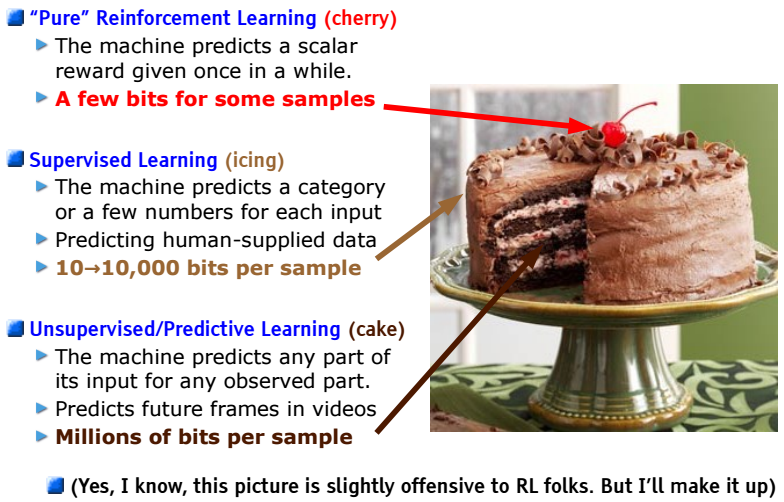
\includegraphics[ scale=.4]{figures/lecunn_icing.png} \\
\end{frame}

\end{document} 